\documentclass[11pt]{article}
\title{\textbf{Meccano frames}}
\author{https://github.com/heptagons/meccano/frames}
\date{}

\usepackage{../meccano}
\usepackage{tikz}
\usetikzlibrary{calc}

\begin{document}

\maketitle
\begin{abstract}
Meccano frames are groups of meccano\meccanoref strips intended to be a
base to build diverse meccano larger objects.
\end{abstract}

\section{Triangle frame with extensions}

\begin{figure}[h]
\centering
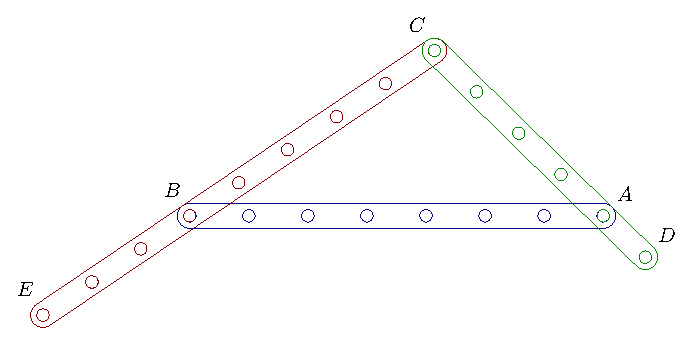
\includegraphics[scale=0.75]{frame_triangle}
\caption{Triangle frame. We have three strips to form the triangle $\triangle{ABC}$.
At least we extend one of two strips $\overline{CB}$ and $\overline{CA}$ to become
$\overline{CE}$ and $\overline{CD}$. The new nodes $D$ and $E$ are rigid and the distance
between them can be a surd, that we can use to be part of more complicated constructions.}
\label{fig:triangle}
\end{figure}

Figure \ref{fig:triangle} is a triangle with extentions. We'll calculate the distance
$\overline{DE}$ to be used as a surd. First we define integer distances $a,b,c,d,e$
and calculate the cosine of $\angle{BCA}$:
\begin{align}
a = \overline{CB}, \quad b = \overline{CA}  \quad c &= \overline{AB}
 \quad d =\overline{BE}, \quad e = \overline{AD} \\
\theta &\equiv \angle{BCA} \\
\cos\theta &= \frac{a^2 + b^2 - c^2}{2ab}
\end{align}
Then we apply the cosine to the triangle $\triangle{CED}$:
\begin{align}
\overline{ED}^2 &= \overline{CD}^2 + \overline{CE}^2
 - 2\overline{CD} \times \overline{CE}\cos\theta \nonumber\\
 &= (a+d)^2 + (b+e)^2 - 2(a+d)(b+e)\cos\theta
\end{align}
So we define the surd $s = \overline{DE}$ as:
\begin{align}
 s &= \sqrt{(a+d)^2 + (b+e)^2 - 2(a+d)(b+e)\cos\theta} \nonumber\\
  &=  \sqrt{(a+d)^2 + (b+e)^2 - 2(a+d)(b+e)\left(\frac{a^2 + b^2 - c^2}{2ab}\right)}
\end{align}

\subsection{Software}

We write a software to find all the triangles with extensions for a particular surd
and for a maximum sides $a+d,b+w,c$.
For example next list show all the $s = \sqrt{7}$
for the three strips $a+d,b+e,c \leq 10$:
\begin{lstlisting}
sqrt{7} max=10
  1) a=1 b+e=1+2 c=1 cos=1/2
  2) a+d=1+1 b+e=1+2 c=1 cos=1/2
  3) a+d=1+2 b=1 c=1 cos=1/2
  4) a+d=1+2 b+e=1+1 c=1 cos=1/2
  5) a=2 b+e=2+1 c=2 cos=1/2
  6) a+d=2+1 b=2 c=2 cos=1/2
  7) a=3 b+e=2+2 c=2 cos=3/4 E=pi/2
  8) a+d=3+1 b+e=2+1 c=2 cos=3/4 D=pi/2
  9) a+d=4+2 b+e=4+4 c=1 cos=31/32
 10) a+d=4+4 b+e=4+2 c=1 cos=31/32
 11) a=7 b+e=5+1 c=3 cos=13/14
 12) a=7 b+e=5+2 c=3 cos=13/14
\end{lstlisting}
The code is in file \texttt{github.com/heptagons/meccano/frames/frames.go}
and function \texttt{func (t *Frames) SurdsInt(surd Z, max N32, frame func(a *FrameSurd))}

\newcommand{\meccanoframetriangle}[5]
{
\begin{tikzpicture}
\def\p {3pt}
\def\a{#1}
\def\b{#2}
\def\c{#3}
\def\d{#4}
\def\e{#5}
\pgfmathsetmacro{\ad}{\a + \d}
\pgfmathsetmacro{\be}{\b + \e}
\pgfmathsetmacro{\cosb}{(\a^2 + \c^2 - \b^2)/(2*\a*\c)}
\pgfmathsetmacro{\cosa}{(\b^2 + \c^2 - \a^2)/(2*\b*\c)}
\begin{scope}
  \meccanostrip[0000cc]{\c}{1}{\p} % blue c=BA
   \begin{scope}[rotate={acos(\cosb)},shift={(-\d,0)}]
    \meccanostrip[cc0000]{\ad}{1}{\p} % red a+d=CB+BE
    \path (0,0) ++(90:5*\p) node{$E$};
    \path (\d,0) ++(90:5*\p) node{$B$};
    \path (\a+\d,0) ++(90:5*\p) node{$C$};
   \end{scope}
   \begin{scope}[shift={(\c,0)},rotate=180-acos{\cosa},shift={(-\e,0)}]
    \meccanostrip[008800]{\be}{1}{\p} % green b+e=CA+AD
    \path (\e,0) ++(-90:5*\p) node{$A$};
    \path (0,0) ++(-90:5*\p) node{$D$};
   \end{scope}
\end{scope}
\end{tikzpicture}
}


\begin{figure}[h]
\centering
\meccanoframetriangle{3}{2}{2}{1}{1}
\caption{Solution for $\overline{DE}=\sqrt{7}$ when $a+d=3+1, b+e=2+1, c=2$.}
\end{figure}


\section{Algebraic distance not right}


\begin{figure}[h]
\centering
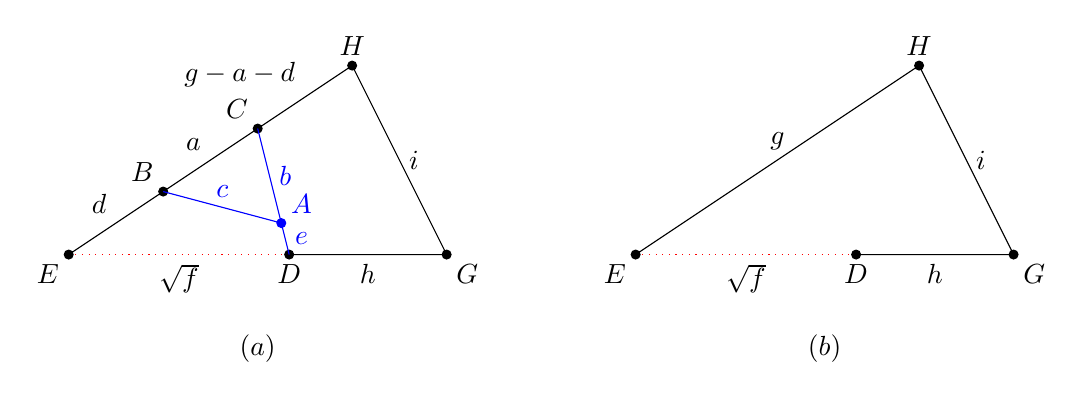
\begin{tikzpicture}
\begin{scope}[scale=0.4]
\begin{scope}
\draw[red,dotted] (0,0) -- node[below,black]{$\sqrt{f}$}++(7,0);
\draw[black,fill=black] (7,0) node[below]{$D$}  circle(4pt)
-- node[below]{$h$} ++(5,0) node[below right]{$G$} circle(4pt)
-- node[right]{$i$} ++(-3,6) node[above]{$H$} circle(4pt)
-- node[above left]{$g-a-d$} ++(-3,-2) node[above left]{$C$} circle(4pt)
-- node[above left]{$a$} ++(-3,-2) node[above left]{$B$} circle(4pt)
-- node[above left]{$d$} ++(-3,-2) node[below left]{$E$} circle(4pt);
\draw[blue,fill=blue] (7,0)
-- node[right]{$e$} ++(-.25,1) node[above right]{$A$} circle(4pt)
-- node[right]{$b$} ++(-.75,3)
   ++(+.75,-3)
-- node[above]{$c$} (3,2);
\draw[black](6,-3) node{$(a)$};

\end{scope}

\begin{scope}[shift={(18,0)}]
\draw[red,dotted] (0,0) -- node[below,black]{$\sqrt{f}$}++(7,0);
\draw[black,fill=black] (7,0) node[below]{$D$}  circle(4pt)
-- node[below]{$h$} ++(5,0) node[below right]{$G$} circle(4pt)
-- node[right]{$i$} ++(-3,6) node[above]{$H$} circle(4pt)
-- node[above]{$g$} ++(-9,-6) node[below left]{$E$} circle(4pt);
\draw[black](6,-3) node{$(b)$};
\end{scope}


\end{scope}
\end{tikzpicture}
\caption{The five strips intented to form an algebraic distance $\sqrt{f} + h$.}
\label{fig:alg-not-right}
\end{figure}

From figure \ref{fig:alg-not-right} $(a)$ we know $\sqrt{f}$ distance
between nodes $E$ and $D$ is produced by the three strips frame $a+d$, $b+e$ and $c$.
Using the law of cosines we calculate the angle $\theta = \angle{CED}$ in terms of $\sqrt{f}$:

\begin{align}
\cos\theta &= \frac{(a+d)^2 + (\sqrt{f})^2 - (b+e)^2}{2(a+d)\sqrt{f}} \nonumber\\
 &= \frac{((a+d)^2 + f - (b+e)^2)\sqrt{f}}{2(a+d)f} \\
 &= \frac{m\sqrt{f}}{n} \label{eq:cos1}\\
 m &= (a+d)^2 + f - (b+e)^2 \\
 n &= 2(a+d)f
\end{align}

From figure \ref{fig:alg-not-right} $(a)$ we notice two sets of points are collinear:
$\{ E,B,C,H \}$ and $\{ E,D,G \}$. Using the law of cosines we calculate the 
angle $\theta = \angle{HEG}$ in terms of distances $g,h,i$:

\begin{align}
\cos\theta &= \frac{g^2 + (\sqrt{f}+h)^2 - i^2}{2g(\sqrt{f}+h)} \nonumber\\
 &= \frac{g^2 + f + 2\sqrt{f}h + h^2 - i^2}{2g(\sqrt{f}+h)} \nonumber\\
 &= \frac{g^2 + f + h^2 - i^2+ 2\sqrt{f}h}{2g(\sqrt{f}+h)}
\end{align}

We multiply both numerator and denominator by $\sqrt{f}-h$ to eliminate the surd from denominator:
\begin{align}
\cos\theta &= \frac{(f + g^2 + h^2 - i^2)(\sqrt{f}-h) + 2\sqrt{f}h(\sqrt{f}-h)}
	{2g(\sqrt{f}+h)(\sqrt{f}-h)} \nonumber\\
 &= \frac{(f + g^2 + h^2 - i^2)(\sqrt{f}-h) + 2fh - 2\sqrt{f}h^2}
	{2g(f-h^2)} \nonumber\\ 
 &= \frac{-h(f + g^2 + h^2 - i^2 - 2f) + (f + g^2 + h^2 - i^2 - 2h^2)\sqrt{f}}
	{2g(f-h^2)} \nonumber\\ 
 &= \frac{h(f - g^2 - h^2 + i^2) + (f + g^2 - h^2 - i^2)\sqrt{f}}
	{2g(f-h^2)} \nonumber\\ 
 &= \frac{o + p\sqrt{f}}{q} \label{eq:cos2}\\
o &= h(f - g^2 - h^2 + i^2) \\
p &= f + g^2 - h^2 - i^2 \\
q &= 2g(f-h^2)
\end{align}

We compare both cosines equations \ref{eq:cos1} and \ref{eq:cos2}:
\begin{align}
\frac{m\sqrt{f}}{n} &= \frac{o + p\sqrt{f}}{q}
\end{align}
Since all variables are integers we need two conditions. First $o$ should be zero.
And second $\frac{m}{n} = \frac{p}{q}$.

For condition 1, we force $o$ to be zero:
\begin{align}
o &= 0 \nonumber\\
h(f - g^2 - h^2 + i^2) & = 0 \nonumber\\
f &= g^2 + h^2 - i^2 \label{eq:condition1}
\end{align}

For condition2, we force $m,n,p,q$ as:
\begin{align}
\frac{m}{n} &= \frac{p}{q} \nonumber\\
\frac{(a+d)^2 + f - (b+e)^2}{2(a+d)f} &= \frac{f + g^2 - h^2 - i^2}{2g(f-h^2)} \nonumber\\
\end{align}

We replace the value of $f$ of last equation RHS with the value of equation \ref{eq:condition1}
of condition 1:
\begin{align}
\frac{(a+d)^2 - (b+e)^2 + f}{(a+d)f} &= \frac{f + g^2 - h^2 - i^2}{g(f-h^2)} \nonumber\\
 &= \frac{g^2 + h^2 - i^2 + g^2 - h^2 - i^2}{g(g^2 + h^2 - i^2-h^2)} \nonumber\\
 &= \frac{2(g^2 - i^2)}{g(g^2 - i^2)} \nonumber\\
 &= \frac{2}{g} \nonumber\\
((a+d)^2 - (b+e)^2 + f)g &= 2(a+d)f \label{eq:condition2}
\end{align}















\end{document}